\documentclass[article,nojss]{jss}
\usepackage{amsmath}

%%%% FIX THESE WHEN YOU REVISE! %%%%%%%%%%%%%%%%
\def\VERSION{2.00}
\def\DATE{5 December 2012}
%%%%%%%%%%%%%%%%%%%%%%%%%%%%%%%%%%%%%%%%%%%%%%%%

\def\rsm{\pkg{rsm}}
\def\R{\proglang{R}}
\def\Sect#1{Section~\ref{#1}}
\def\bb{\mathbf{b}}
\def\bB{\mathbf{B}}
\def\bu{\mathbf{u}}
\def\bU{\mathbf{U}}
\def\bLambda{\pmb{\Lambda}}
\def\bgamma{\pmb{\gamma}}
\def\bx{\mathbf{x}}
\def\bzero{\mathbf{0}}
\def\yhat{\hat{y}}
\def\bmat#1{\begin{bmatrix}#1\end{bmatrix}}

%% need no \usepackage{Sweave}

\IfFileExists{upquote.sty}{\RequirePackage{upquote}}{}
\DefineShortVerb{\"}

%\VignetteIndexEntry{Response-Surface Methods in R, Using rsm}
%\VignetteDepends{rsm}
%\VignetteKeywords{response-surface methods, regression, experimental design, first-order designs, second-order designs}
%\VignettePackage{rsm}

\author{Russell V.~Lenth\\The University of Iowa}
\Plainauthor{Russell V. Lenth}

\title{Response-Surface Methods in \proglang{R}, Using \pkg{rsm}\\
\normalsize Updated to version \VERSION, \DATE}
\Plaintitle{Response-Surface Methods in R, Using rsm}

\Abstract{
  This introduction to the \proglang{R} package \pkg{rsm} is a
  modified version of \cite{Lenth:2009}, published in the
  \emph{Journal of Statistical Software}. The package \rsm{}  
  was designed to
  provide \R{} support for standard response-surface methods.  Functions are
  provided to generate central-composite and Box-Behnken designs.  For analysis
  of the resulting data, the package provides for estimating the response
  surface, testing its lack of fit, displaying an ensemble of contour plots of
  the fitted surface, and doing follow-up analyses such as steepest ascent,
  canonical analysis, and ridge analysis.  It also implements a coded-data
  structure to aid in this essential aspect of the methodology.  The functions
  are designed in hopes of providing an intuitive and effective user interface. 
  Potential exists for expanding the package in a variety of ways.
}

\Keywords{response-surface methods, regression, experimental design, first-order designs, second-order designs}

\Address{
  Russell V.~Lenth\\
  Department of Statistics\\
  The University of Iowa\\
  Iowa City, IA 52242, United States of America\\
  E-mail: \email{russell-lenth@uiowa.edu}\\
  URL: \url{http://www.stat.uiowa.edu/~rlenth/}
}


\begin{document}

\section{Introduction}
Response-surface methodology comprises a body of methods for exploring for optimum operating conditions through experimental methods.  Typically, this involves doing several experiments, using the results of one experiment to provide direction for what to do next.  This next action could be to focus the experiment around a different set of conditions, or to collect more data in the current experimental region in order to fit a higher-order model or confirm what we seem to have found.  

Different levels or values of the operating conditions comprise the factors in each experiment.  Some may be categorical (e.g., the supplier of raw material) and others may be quantitative (feed rates, temperatures, and such).  In practice, categorical variables must be handled separately by comparing our best operating conditions with respect to the quantitative variables across different combinations of the categorical ones.  The fundamental methods for quantitative variables involve fitting first-order (linear) or second-order (quadratic) functions of the predictors to one or more response variables, and then examining the characteristics of the fitted surface to decide what action is appropriate.

Given that, it may seem like response-surface analysis is simply a regression problem.  However, there are several intricacies in this analysis and in how it is commonly used that are enough different from routine regression problems that some special help is warranted.  These intricacies include the common use (and importance) of coded predictor variables; the assessment of the fit; the different follow-up analyses that are used depending on what type of model is fitted, as well as the outcome of the analysis; and the importance of visualizing the response surface.  Response-surface methods also involve some unique experimental-design issues, due to the emphasis on iterative experimentation and the need for relatively sparse designs that can be built-up piece-by-piece according to the evolving needs of the experimenter.

The \rsm{} package for \R{} \citep{R} provides several functions to facilitate classical response-surface methods, as
described in texts such as \cite{Box87}, \citet[Chapters~1--5]{Khu96}, \citet[Chapter~9]{Wu00}, \cite{Mye09},
\citet[Chapters~11--12]{Box05}, and \citet[Chapter~10]{Ryan07}.  In its current form, \rsm{} covers only the
most standard first-and second order designs and methods for one response variable; but it covers those
reasonably well, and it could be expanded in the future.  Multiple-response optimization is not covered
in this package, but the \pkg{desirability} package \cite[]{Kuh09} may be used in conjunction with
predictions obtained using the \rsm{} package. The \rsm{} package is available from the Comprehensive
\proglang{R} Archive Network at \url{http://CRAN.R-project.org/package=rsm}.

Here is a general overview of \rsm{}.  First, it provides functions and data types that provide for the coding and decoding of factor levels, since appropriate coding is an important element of response-surface analysis.  These are discussed in \Sect{coding}.  Second, it provides functions for generating standard designs (currently, central-composite and Box-Behnken), and building blocks thereof, and examining their variance function; see \Sect{designs}.  Third (\Sect{fitting}), it extends \R's "lm" function to simplify the specification of standard response-surface models, and provide appropriate summaries.  Fourth (\Sect{contour}) it provides means of visualizing a fitted response surface (or in fact any "lm" object).  Finally (\Sect{steepest}), it provides guidance for further experimentation, e.g., along the path of steepest ascent.  Most \rsm{} functions take advantage of \R's formula capabilities to provide intuitive and transparent ways of obtaining the needed results.

To provide some context, there is good commercial software available to help with designing and analyzing
response-surface experiments.  The most popular include \pkg{Design-Expert}~\citep{DEsoft},
\pkg{JMP}~\citep{JMPsoft}, and~\pkg{Statgraphics}~\citep{SGsoft}.  These all provide for generating Box-Behnken and central-composite designs, fitting first- and second-order response surfaces, and visualizing them.  These programs generally exceed \rsm's capabilities (for example, more types of designs, provisions for mixture experiments, etc.); but \rsm{} makes the most important methods available in \R.  To my knowledge, the functionality of \rsm's "ccd.pick" function is not provided in other software, and \rsm{} may exceed the capabilities of these programs in the generality of central-composite designs that it can create.

The goal of this article is to present an overview of \rsm{} and how its functions may be used to design and analyze response-surface experiments.  While most important functions in the package are illustrated, we do not provide comprehensive documentation here; instead, the reader is referred to the manual and online documentation provided with the package. Further note that \pkg{rsm}'s features were extended and somewhat modified in version 2.0, and the vignette \href{rs-illus.pdf}{``Response-Surface Illustration''} illustrates using the newer building-block approach to generating designs and some other newer features.



\section{Coding of data}\label{coding}
An important aspect of response-surface analysis is using an appropriate coding transformation of the data.  The way the data are coded affects the results of canonical analysis (see \Sect{fitting}) and steepest-ascent analysis (see \Sect{steepest}); for example, unless the scaling factors are all equal, the path of steepest ascent obtained by fitting a model to the raw predictor values will differ from the path obtained in the coded units, decoded to the original scale.  Using a coding method that makes all coded variables in the experiment vary over the same range is a way of giving each predictor an equal share in potentially determining the steepest-ascent path.  Thus, coding is an important step in response-surface analysis.

Accordingly, the \rsm{} package provides for a "coded.data" class of objects, an extension of "data.frame".  The functions "coded.data", "as.coded.data", "decode.data", "recode.data", "code2val", and "val2code" create or decode such objects.  If a "coded.data" object is used in place of an ordinary "data.frame" in the call to other \rsm{} functions such as "rsm" (\Sect{fitting}) or "steepest" (\Sect{steepest}), then appropriate additional output is provided that translates the results to the original units.  The print method for a "coded.data" object displays the coding formulas and the data in either coded or decoded form.

As an example, consider the provided dataset "ChemReact", which comes from Table~7.6 of \cite{Mye09}.
\begin{Schunk}
\begin{Sinput}
R> library("rsm")
R> ChemReact
\end{Sinput}
\begin{Soutput}
    Time   Temp Block Yield
1  80.00 170.00    B1  80.5
2  80.00 180.00    B1  81.5
3  90.00 170.00    B1  82.0
4  90.00 180.00    B1  83.5
5  85.00 175.00    B1  83.9
6  85.00 175.00    B1  84.3
7  85.00 175.00    B1  84.0
8  85.00 175.00    B2  79.7
9  85.00 175.00    B2  79.8
10 85.00 175.00    B2  79.5
11 92.07 175.00    B2  78.4
12 77.93 175.00    B2  75.6
13 85.00 182.07    B2  78.5
14 85.00 167.93    B2  77.0
\end{Soutput}
\end{Schunk}
In this experiment, the data in block "B1" were collected first and analyzed, after which block "B2" was added and a new analysis was done. The provided datasets "ChemReact1" and "ChemReact2" provide these separate blocks. 
The first block, "ChemReact1", uses factor settings of $\text{Time}=85\pm5$ and $\text{Temp}=175\pm5$, with three center points.  Thus, the coded variables are $x_1 = (\text{Time}-85)/5$ and $x_1 = (\text{Temp}-175)/5$.  To create a coded dataset with the appropriate codings, provide this information via formulas:
\begin{Schunk}
\begin{Sinput}
R> CR1 <- coded.data(ChemReact1, x1 ~ (Time - 85)/5, x2 ~ (Temp - 175)/5)
R> CR1
\end{Sinput}
\begin{Soutput}
  Time Temp Yield
1   80  170  80.5
2   80  180  81.5
3   90  170  82.0
4   90  180  83.5
5   85  175  83.9
6   85  175  84.3
7   85  175  84.0

Data are stored in coded form using these coding formulas ...
x1 ~ (Time - 85)/5
x2 ~ (Temp - 175)/5
\end{Soutput}
\end{Schunk}
This listing looks much like the original data, but internally, the data are saved in coded form, as can be seen by coercing it to a "data.frame":
\begin{Schunk}
\begin{Sinput}
R> as.data.frame(CR1)
\end{Sinput}
\begin{Soutput}
  x1 x2 Yield
1 -1 -1  80.5
2 -1  1  81.5
3  1 -1  82.0
4  1  1  83.5
5  0  0  83.9
6  0  0  84.3
7  0  0  84.0
\end{Soutput}
\end{Schunk}
Any way of writing a linear transformation is acceptable; for example, we could have written "x1 ~ 0.2 * Time - 17".
Observe that "coded.data" actually transforms the predictor values and replaces those variables with their coded versions.  To create a "coded.data" object from data that are already coded, use "as.coded.data".

%!======================================================================
%!=====================================================================


The function "decode.data" decodes a "coded.data" object.  We may also easily encode or decode matrices or data frames of arbitrary values; for example,
\begin{Schunk}
\begin{Sinput}
R> code2val(data.frame(x1 = c(0.25, 0.5), x2 = c(-1.5, -0.5)), codings(CR1))
\end{Sinput}
\begin{Soutput}
   Time  Temp
1 86.25 167.5
2 87.50 172.5
\end{Soutput}
\end{Schunk}


\section{Generating a design}\label{designs}
The functions "ccd" and "bbd" are available to generate standard response-surface designs.  For example, here
we generate a 3-factor Box-Behnken design \cite[]{Box60} with two center points:
\begin{Schunk}
\begin{Sinput}
R> bbd(3, n0 = 2, coding =
+   list(x1 ~ (Force - 20)/3, x2 ~ (Rate - 50)/10, x3 ~ Polish - 4))
\end{Sinput}
\begin{Soutput}
   run.order std.order Force Rate Polish
1          1         4    23   60      4
2          2         2    23   40      4
3          3         5    17   50      3
4          4         6    23   50      3
5          5        10    20   60      3
6          6        14    20   50      4
7          7        12    20   60      5
8          8         3    17   60      4
9          9         9    20   40      3
10        10         8    23   50      5
11        11         1    17   40      4
12        12         7    17   50      5
13        13        11    20   40      5
14        14        13    20   50      4

Data are stored in coded form using these coding formulas ...
x1 ~ (Force - 20)/3
x2 ~ (Rate - 50)/10
x3 ~ Polish - 4
\end{Soutput}
\end{Schunk}
By default, the variable names are "x1", "x2", \ldots and the experiment is randomized.  If there are $4$ or $5$ factors, the design is blocked by default (this is not possible for other numbers of factors), and the blocks are randomized separately.


One of the most popular response-surface designs is the central-composite design (CCD), due to \cite{Box51}.  A simple example is the chemical-reaction experiment presented in the preceding section.  These designs allow for sequential augmentation, so that we may first experiment with just one block suitable for fitting a first-order model, and then add more block(s) if a second-order fit is needed.  
The blocks in a CCD are of two types---one type, called a ``cube'' block, contains design points from a two-level factorial or fractional factorial design, plus center points; the other type, called a ``star'' block, contains axis points plus center points.  

In the following discussion, the term ``design points'' refers to the non-center points in a block.  The levels of the factors are coded, so that the cube blocks contain design points with coordinate values all equal to $\pm1$, and center points at $(0,0,\ldots,0)$.  The design points in the star blocks are at positions of $\pm\alpha$ along each coordinate axis.  The value of $\alpha$, and choices of replications of design points and center points, are often selected based on considerations of rotatability (i.e., the variance of the prediction depends only on the distance from the center) and orthogonality of blocks (so that the coefficients of the fitted response-surface equation are not correlated with block effects).

\begin{table}[t!]
\begin{center}
\def\arraystretch{1.5}
\begin{tabular}{|p{1.72in}|c|c|}
\hline
Parameter(s) & Cube block(s) & Star block(s) \\ 
\hline
Design points & $(\pm1,\pm1,\ldots,\pm1)$
    & $(\pm\alpha,0,0,\ldots,0),\ldots,(0,0,\ldots,\pm\alpha)$ \\
Center points & $(0,0,\ldots,0)$ & $(0,0,\ldots,0)$ \\ 
\hline
\# \emph{Distinct} design points 
  & $2^{k-p}$ (altogether)
  & $2k$\\
%%%%%\hline
\# Fractions of $2^{k-p}$
  & \texttt{blks.c}  & (Not applicable)\\
Reps of each design point, within each block
  & \texttt{wbr.c} & \texttt{wbr.s} \\
\# Design pts each block
  & \texttt{n.c} $= \mathtt{\frac{wbr.c}{blks.c}}\cdot2^{k-p}$
  & n.s $=\mathtt{wbr.s}\cdot(2k)$\\
\# Center points 
  & \texttt{n0.c}  & \texttt{n0.s}\\
\# Points in each block
  & \texttt{n.c + n0.c}
  & \texttt{n.s + n0.s} \\
Reps of each block
  & \texttt{bbr.c} & \texttt{bbr.s}\\
  \hline
Total observations (\texttt{N})
  & \multicolumn{2}{|c|}{\tt \parbox{174pt}{blks.c * bbr.c * (n.c + n0.c) + bbr.s * (n.s + n0.s)}\rule[-16pt]{0pt}{36pt}}\\
\hline
\end{tabular}
\caption{\label{ccd-ref} Parameters of a central-composite design, and names used by \texttt{ccd.pick}.}
\end{center}
\end{table}

Table~\ref{ccd-ref} displays the parameters of a CCD, along with the names used by the function "ccd.pick" to be described shortly.  Suppose that there are $k$ variables to be varied.  For the cube blocks, we start with a given $2^{k-p}$ fractional factorial design (or full factorial, when $p=0$).  We may either use this design as-is to define the design points in the cube block(s).  Alternatively, we may confound one or more effects with blocks to split this design into "blks.c" smaller cube blocks, in which case each cube block contains $2^{k-p}/\mathtt{blks.c}$ distinct design points.  The star blocks always contain all $2k$ distinct design points---two on each axis.

Once the designs are decided, we may, if we like, replicate them within blocks.  We may also replicate the center points.  The names "wbr.c" and "wbr.s" (for ``within-block reps'') refer to the number of replicates of each design point within each cube block or star block, respectively.  
Thus, each cube block has a total of $\mathtt{n.c} = \mathtt{wbr.c}\cdot2^{k-p}/\mathtt{blks.c}$ design points, and each star block contains $\mathtt{wbr.s}\cdot2k$ design points.
We may also replicate the center points---"n0.c" times in each cube block, "n0.s" times within each star block.

Finally, we may replicate the blocks themselves; the numbers of such between-block replications are denoted "bbr.c" and~"bbr.s" for cube blocks and star blocks, respectively.  It is important to understand that each block is separately randomized, in effect a mini-experiment within the larger experiment.  Having between-block replications means repeating these mini-experiments.  We run an entire block before running another block. 

The function "ccd.pick" is designed to help identify good CCDs.  It simply creates a grid of all combinations of design choices, computes the $\alpha$ values required for orthogonality and rotatability, sorts them by a specified criterion (by default, a measure of the discrepancy between these two $\alpha$s), and presents the best few.  

For example, suppose that we want to experiment with $k=5$ factors, and we are willing to consider CCDs with $\mathtt{blks.c}=1$, $2$, or $4$ cube blocks of sizes $\mathtt{n.c}=8$ or $16$ each.  
With this many factors, the number of different star points ($2k=10$) is relatively small compared with the size of some cube blocks ($16$), so it seems reasonable to consider either one or two replications ($\mathtt{wbr.s}\in\{1,2\}$) of each point within each star block.  
Finally, suppose that we want the total size of the experiment to be no more than $N=65$ runs (see "restrict" in the call below).  Here are the ten best choices based on these criteria:
\begin{Schunk}
\begin{Sinput}
R> ccd.pick(5, n.c = c(8, 16), blks.c = c(1, 2, 4),
+   wbr.s = 1:2, restrict = "N<=65")
\end{Sinput}
\begin{Soutput}
   n.c n0.c blks.c n.s n0.s bbr.c wbr.s bbr.s  N alpha.rot alpha.orth
1   16    6      1  10    1     1     1     1 33  2.000000   2.000000
2   16    8      1  10    2     1     1     1 36  2.000000   2.000000
3   16   10      1  10    3     1     1     1 39  2.000000   2.000000
4   16    5      2  20    1     1     2     1 63  2.000000   2.000000
5   16    8      2  10    7     1     1     1 65  2.378414   2.380476
6    8    4      4  10    7     1     1     1 65  2.378414   2.380476
7   16    1      2  10    2     1     1     1 46  2.378414   2.376354
8   16    5      2  10    5     1     1     1 57  2.378414   2.390457
9   16    4      2  10    4     1     1     1 54  2.378414   2.366432
10   8    2      4  10    4     1     1     1 54  2.378414   2.366432
\end{Soutput}
\end{Schunk}
The first design listed is also the smallest; it consists of one cube block of $16$ runs, plus $6$ center points; and one star block with the points replicated once and one center point; thus, the total number of runs is $N=(16+6)+(10+1) = 33$.
If we choose $\alpha=2$, this design is both orthogonal and rotatable as seen by noting that "alpha.rot" and "alpha.orth" are both equal to $2$.  The $16$ design points in the cube block may be generated by a $2^{5-1}$ fractional factorial design.

While this is a small design, we have only one center point in the star block, not providing a way to test lack of fit in the star portion.  The second and third designs remedy this slightly, but all these designs are fairly lopsided in that the cube block is much larger than the star block.  The next few designs require considerably more runs.  Design number~4 is nicely balanced in that it consists of three blocks of $21$ runs each, and it is both rotatable and orthogonal.  However, we still have no lack-of-fit test in the star blocks.  Designs 5 and~6 differ only in whether they use two $2^{5-1}$ cubes or four $2^{5-2}$ cubes, but they provide several center points for a lack-of-fit test.  If we position the axis points at $\alpha=2.38$, the design is almost orthogonal and almost rotatable.  The remaining designs also come close to meeting both criteria, but are also somewhat smaller, so that Designs 9 and~10 are essentially down-sized versions of Designs 5 and~6.

The choice of which design is best depends on the tradeoff between economy and ability to assess the fitted surface.  Design~1 is the only one of these that is included in Table~7.6 of \cite{Mye09}.  It is good to be able to look at a broader range of choices.

Once we decide the design, the "ccd" function is used to generate it. (Alternatively, starting with \pkg{rsm} version 2.0, the "cube", "star", "foldover", and "dupe" functions are available for generating and randomizing a CCD in separate blocks, and then they may be combined using "djoin".)
We first illustrate the generation of Design~1 above.  This design requires a $2^{5-1}$ fraction for the cube block.  Typically, this is done by confounding the five-way interaction with the mean; or equivalently, create a four-factor design, and generate the levels of the fifth as the four-way interaction of the others.  That is the approach implemented by "ccd".
Suppose that we denote the design factors by $A,B,C,D,E$; let's opt to use $E=-ABCD$ as the generator.  The following call generates the design (results not shown):
\begin{Schunk}
\begin{Sinput}
R> des1 <- ccd (y1 + y2 ~ A + B + C + D,
+   generators = E ~ - A * B * C * D, n0 = c(6, 1))
\end{Sinput}
\end{Schunk}
The value of $\alpha$ was not specified, and by default it uses the $\alpha$ for orthogonality.  The first argument could have been just "4", but then the generator would have had to have been given in terms of the default variable names "x1", "x2", \ldots.  The optional left-hand side in the formula creates place-holders for response variable(s), to be filled-in with data later.  As in "bbd", we could have added coding formulas to create a "coded.data" object. 

Next, we illustrate the generation of Design~10.
This design has four $2^{5-2}$ cube blocks with $2$ center points each, and one unreplicated star block with $4$ center points.  The non-center points in the cube blocks comprise $4\times8=32$ runs, so we most likely want to create them by dividing the full $2^5$ factorial into four fractional blocks.  We can for example opt to generate the blocks via the factors $b_1=ABC$ and $b_2=CDE$, so that the blocks are determined by the four combinations of $b_1$ and $b_2$.  Then the block effects will be confounded with the effects $ABC$, $CDE$, and also the $b_1b_2$ interaction $ABC^2DE=ABDE$.  It  is important in response-surface work to avoid confounding second-order interactions, and this scheme is thus acceptable.  Unlike Design~1, this design includes all $2^5$ factor combinations, so we do not use the "generators" argument; instead, we use "blocks" to do the fractionation:
\begin{Schunk}
\begin{Sinput}
R> des10 <- ccd( ~ A + B + C + D + E,
+   blocks = Blk ~ c(A * B * C, C * D * E), n0 = c(2, 4))
\end{Sinput}
\end{Schunk}
Each block is randomized separately, but the order of the blocks is not randomized. In practice, we may opt to run the blocks in a different sequence.  
With this design, just one of the cube blocks is sufficient to estimate a first-order response surface.

It is also important to examine a design's capabilities. First of all, is it adequate to fit the needed first- or second-order model, and how effective is it in predicting the response surface? The "varfcn" function (a new addition starting \pkg{rsm} version 2.0) is helpful in this regard. It calculates a scaled version of the varaince of the fitted values over a specified set of design points. By default, it computes this along paths through $(1,0,\ldots,0),(1,1,\ldots,0),\ldots,(1,1,\ldots,1)$, or on a grid with the first two variables. The right-hand side of the intended model must be provided. 
\begin{figure}
{\small
\begin{Schunk}
\begin{Sinput}
R> par(mfrow=c(1,2))
R> varfcn(des10, ~ Blk + SO(A,B,C,D,E), dist = seq(0, 3, by=.1))
R> varfcn(des10, ~ Blk + SO(A,B,C,D,E), dist = seq(0, 3, by=.1), contour = TRUE)
\end{Sinput}
\end{Schunk}
}
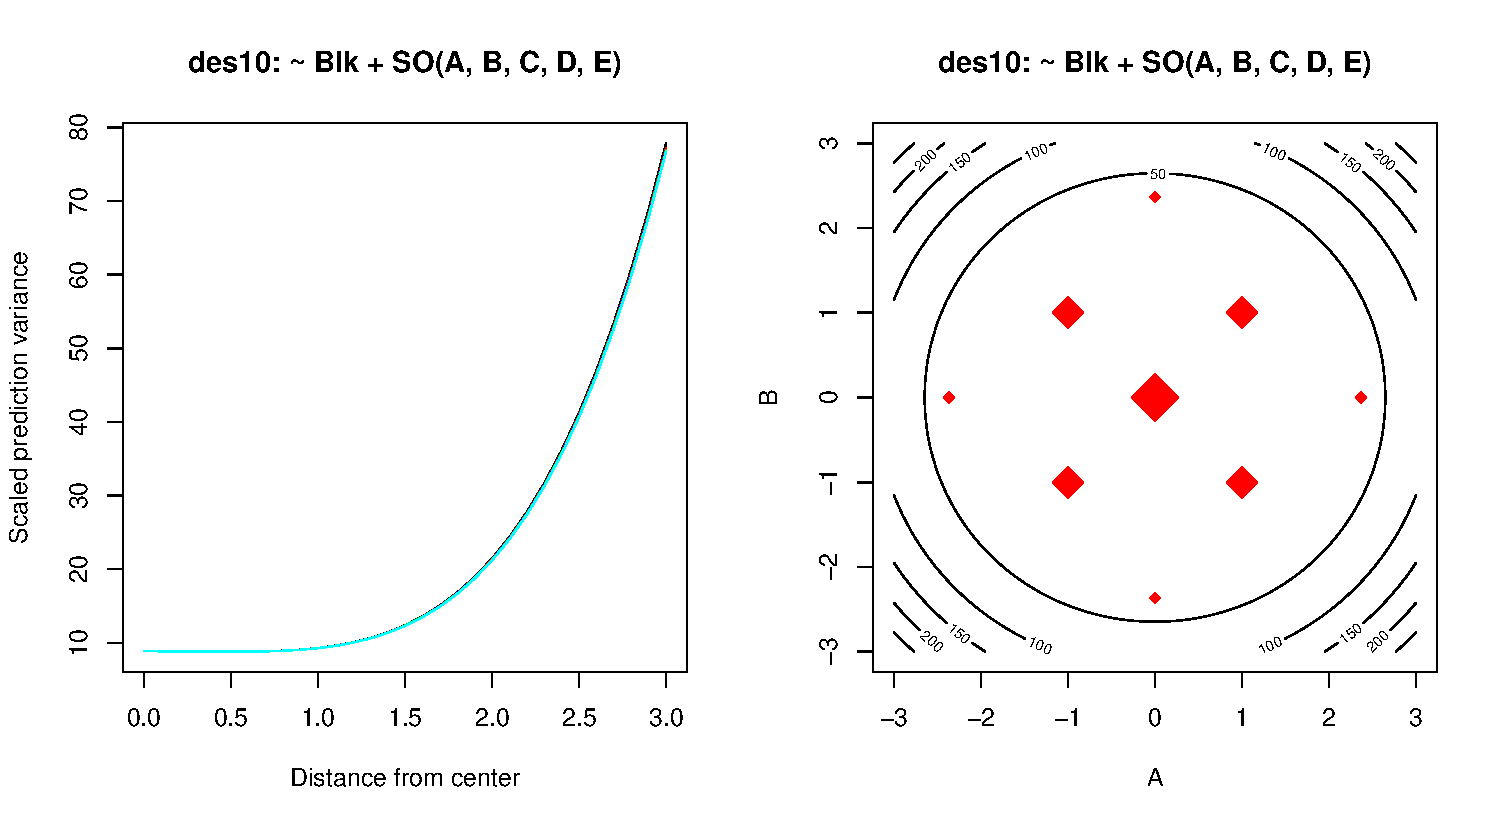
\includegraphics[width=.8\textwidth]{rsm-varfcn.pdf}
\caption{Variance function plots for \code{des10}, with respect to a second-order model.}\label{varfcn}
\rule{18pt}{0pt}\hrule
\end{figure}

Figure~\ref{varfcn} illustrates this for "des10".
It shows that the design is nearly rotatable (it would be exactly so if we had chosen \verb|alpha = "rotatable"| in the call to "ccd").
It can also be verified that any two of the cube blocks plus the axis block is sufficient
to estimate a second-order response surface. Just one cube block plus the axis points, however, is not sufficient.

It is possible to imagine a CCD that consists of a fractional factorial divided into blocks.  For such a design, both "generators" and "blocks" would be needed.  For smaller numbers of factors, most CCDs require no fractionation of either type, and obviously these are simple to generate.

Starting in version~1.40 of \rsm{}, an "inscribed" argument is available in "ccd".  This scales the entire design so that it fits within a unit cube---useful for situations when there are constraints on the region of operability.
\begin{Schunk}
\begin{Sinput}
R> ccd(2, n0 = c(1,1), inscribed=TRUE, randomize=FALSE)
\end{Sinput}
\begin{Soutput}
   run.order std.order   x1.as.is   x2.as.is Block
1          1         1 -0.7071068 -0.7071068     1
2          2         2  0.7071068 -0.7071068     1
3          3         3 -0.7071068  0.7071068     1
4          4         4  0.7071068  0.7071068     1
5          5         5  0.0000000  0.0000000     1
6          1         1 -1.0000000  0.0000000     2
7          2         2  1.0000000  0.0000000     2
8          3         3  0.0000000 -1.0000000     2
9          4         4  0.0000000  1.0000000     2
10         5         5  0.0000000  0.0000000     2

Data are stored in coded form using these coding formulas ...
x1 ~ x1.as.is
x2 ~ x2.as.is
\end{Soutput}
\end{Schunk}
Note in this example that it is now the axis points that are at $\pm1$, while the cube points are at $\pm\sqrt{1/2}$. (Incidentally, this example also illustrates the default codings used when no coding formulas are specified.)

There are several other types of designs that are useful for response surfaces, as mentioned in several of the books referenced in this article.  Provisions for generating those designs are an area of future development in the \rsm{} package.



\section{Fitting a response-surface model}\label{fitting}
A response surface is fitted using the "rsm" function.  This is an extension of "lm", and works almost exactly like it; however, the model formula for "rsm" must make use of the special functions "FO", "TWI", "PQ", or "SO" (for ``first-order,'', ``two-way interaction,'' ``pure quadratic,'' and ``second-order,'' respectively), because the presence of these specifies the response-surface portion of the model.  Other terms that don't involve these functions may be included in the model; often, these terms would include blocking factors and other categorical predictors.

To illustrate this, let us revisit the "ChemReact" data introduced in \Sect{coding}.  We have one response variable, "Yield", and two coded predictors "x1" and "x2" as well as a blocking factor "Block".  Supposing that the experiment was done in two stages, we first act as though the data in the second block have not yet been collected; and fit a first-order response-surface model to the data in the first block:
\begin{Schunk}
\begin{Sinput}
R> CR1.rsm <- rsm(Yield ~ FO(x1, x2), data = CR1)
R> summary(CR1.rsm)
\end{Sinput}
\begin{Soutput}
Call:
rsm(formula = Yield ~ FO(x1, x2), data = CR1)

            Estimate Std. Error  t value  Pr(>|t|)    
(Intercept) 82.81429    0.54719 151.3456 1.143e-08 ***
x1           0.87500    0.72386   1.2088    0.2933    
x2           0.62500    0.72386   0.8634    0.4366    
---
Signif. codes:  0 '***' 0.001 '**' 0.01 '*' 0.05 '.' 0.1 ' ' 1 

Analysis of Variance Table

Response: Yield
            Df Sum Sq Mean Sq F value  Pr(>F)
FO(x1, x2)   2 4.6250  2.3125  1.1033 0.41534
Residuals    4 8.3836  2.0959                
Lack of fit  2 8.2969  4.1485 95.7335 0.01034
Pure error   2 0.0867  0.0433                

Direction of steepest ascent (at radius 1):
       x1        x2 
0.8137335 0.5812382 

Corresponding increment in original units:
    Time     Temp 
4.068667 2.906191 
\end{Soutput}
\end{Schunk}
What we see in the summary is the usual summary for a "lm" object (with a subtle difference), followed by some additional information particular to response surfaces.  The subtle difference is that the labeling of the regression coefficients is simplified (we don't see ``"FO"'' in there).  The analysis-of-variance table shown includes a breakdown of lack of fit and pure error, and we are also given information about the direction of steepest ascent.  Since the dataset is a "coded.data" object, the steepest-ascent information is also presented in original units.  (While "rsm" does not require a "coded.data" dataset, the use of one is highly recommended.)

In this particular example, the steepest-ascent information is of little use, because there is significant
lack of fit for this model ($p \approx 0.01$).  It suggests that we should try a higher-order model.  For example, we could add two-way interactions:
\begin{Schunk}
\begin{Sinput}
R> CR1.rsmi <- update(CR1.rsm, . ~ . + TWI(x1, x2))
R> summary(CR1.rsmi)
\end{Sinput}
\end{Schunk}
The results are not shown, but one finds there is still a small $p$~value for lack-of-fit.  

To go further, we need more data.  Thus, let us pretend that we now collect the data in the second block. 
Then here are the data from the combined blocks:
\begin{Schunk}
\begin{Sinput}
R> ( CR2 <- djoin(CR1, ChemReact2) )
\end{Sinput}
\begin{Soutput}
    Time   Temp Yield Block
1  80.00 170.00  80.5     1
2  80.00 180.00  81.5     1
3  90.00 170.00  82.0     1
4  90.00 180.00  83.5     1
5  85.00 175.00  83.9     1
6  85.00 175.00  84.3     1
7  85.00 175.00  84.0     1
8  85.00 175.00  79.7     2
9  85.00 175.00  79.8     2
10 85.00 175.00  79.5     2
11 92.07 175.00  78.4     2
12 77.93 175.00  75.6     2
13 85.00 182.07  78.5     2
14 85.00 167.93  77.0     2

Data are stored in coded form using these coding formulas ...
x1 ~ (Time - 85)/5
x2 ~ (Temp - 175)/5
\end{Soutput}
\end{Schunk}
Notice that "djoin" figures out the fact that "ChemReact2" is not coded but it has the appropriate uncoded variables "Time" and~"Temp"; so it codes those variables appropriately. Also, the "Block" factor is added automatically.

We are now in the position of fitting a full second-order model to the combined data.  This can be done by adding "PQ(x1, x2)" to the above model with interaction, but the easier way is to use "SO", which is shorthand for a model with "FO", "TWI", and "PQ" terms.  Also, we now need to account for the block effect since the data are collected in separate experiments:
\begin{Schunk}
\begin{Sinput}
R> CR2.rsm <- rsm(Yield ~ Block + SO(x1, x2), data = CR2)
R> summary(CR2.rsm)
\end{Sinput}
\begin{Soutput}
Call:
rsm(formula = Yield ~ Block + SO(x1, x2), data = CR2)

             Estimate Std. Error  t value  Pr(>|t|)    
(Intercept) 84.095427   0.079631 1056.067 < 2.2e-16 ***
Block2      -4.457530   0.087226  -51.103 2.877e-10 ***
x1           0.932541   0.057699   16.162 8.444e-07 ***
x2           0.577712   0.057699   10.012 2.122e-05 ***
x1:x2        0.125000   0.081592    1.532    0.1694    
x1^2        -1.308555   0.060064  -21.786 1.083e-07 ***
x2^2        -0.933442   0.060064  -15.541 1.104e-06 ***
---
Signif. codes:  0 '***' 0.001 '**' 0.01 '*' 0.05 '.' 0.1 ' ' 1 

Analysis of Variance Table

Response: Yield
            Df Sum Sq Mean Sq   F value    Pr(>F)
Block        1 69.531  69.531 2611.0950 2.879e-10
FO(x1, x2)   2  9.626   4.813  180.7341 9.450e-07
TWI(x1, x2)  1  0.063   0.063    2.3470    0.1694
PQ(x1, x2)   2 17.791   8.896  334.0539 1.135e-07
Residuals    7  0.186   0.027                    
Lack of fit  3  0.053   0.018    0.5307    0.6851
Pure error   4  0.133   0.033                    

Stationary point of response surface:
       x1        x2 
0.3722954 0.3343802 

Stationary point in original units:
     Time      Temp 
 86.86148 176.67190 

Eigenanalysis:
$values
[1] -0.9233027 -1.3186949

$vectors
         [,1]       [,2]
x1 -0.1601375 -0.9870947
x2 -0.9870947  0.1601375
\end{Soutput}
\end{Schunk}
The lack of fit is now non-significant ($p \approx 0.69$).   The summary for a second-order model provides
results of a canonical analysis of the surface rather than for steepest ascent.  The analysis indicates that
the stationary point of the fitted surface is at $(0.37, 0.33)$ in coded units---well within the experimental region; and that both eigenvalues are negative, indicating that the stationary point is a maximum.  This is the kind of situation we dream for in response-surface experimentation---clear evidence of a nearby set of optimal conditions.  We should probably collect some confirmatory data near this estimated optimum at $\text{Time}\approx87$, $\text{Temp}\approx 177$, to make sure.

Another example that comes out a different way is a paper-helicopter experiment \cite[Table 12.5]{Box05}.  This is another central-composite experiment, in four variables and two blocks.  The data are provided in the \rsm{} dataset "heli"; these data are already coded.  The original variables are wing area "A", wing shape "R", body width "W", and body length "L".  The goal is to make a paper helicopter that flies for as long as possible.  Each observation in the dataset represents the results of ten replicated flights at each experimental condition.  Here we study the average flight time, variable name "ave", using a second-order surface.
\begin{Schunk}
\begin{Sinput}
R> heli.rsm <- rsm(ave ~ block + SO(x1, x2, x3, x4), data = heli)
R> summary(heli.rsm)
\end{Sinput}
\begin{Soutput}
Call:
rsm(formula = ave ~ block + SO(x1, x2, x3, x4), data = heli)

              Estimate Std. Error  t value  Pr(>|t|)    
(Intercept) 372.800000   1.506375 247.4815 < 2.2e-16 ***
block2       -2.950000   1.207787  -2.4425 0.0284522 *  
x1           -0.083333   0.636560  -0.1309 0.8977075    
x2            5.083333   0.636560   7.9856 1.398e-06 ***
x3            0.250000   0.636560   0.3927 0.7004292    
x4           -6.083333   0.636560  -9.5566 1.633e-07 ***
x1:x2        -2.875000   0.779623  -3.6877 0.0024360 ** 
x1:x3        -3.750000   0.779623  -4.8100 0.0002773 ***
x1:x4         4.375000   0.779623   5.6117 6.412e-05 ***
x2:x3         4.625000   0.779623   5.9324 3.657e-05 ***
x2:x4        -1.500000   0.779623  -1.9240 0.0749257 .  
x3:x4        -2.125000   0.779623  -2.7257 0.0164099 *  
x1^2         -2.037500   0.603894  -3.3739 0.0045424 ** 
x2^2         -1.662500   0.603894  -2.7530 0.0155541 *  
x3^2         -2.537500   0.603894  -4.2019 0.0008873 ***
x4^2         -0.162500   0.603894  -0.2691 0.7917877    
---
Signif. codes:  0 '***' 0.001 '**' 0.01 '*' 0.05 '.' 0.1 ' ' 1 

Analysis of Variance Table

Response: ave
                    Df  Sum Sq Mean Sq F value    Pr(>F)
block                1   16.81   16.81  1.7281  0.209786
FO(x1, x2, x3, x4)   4 1510.00  377.50 38.8175 1.965e-07
TWI(x1, x2, x3, x4)  6 1114.00  185.67 19.0917 5.355e-06
PQ(x1, x2, x3, x4)   4  282.54   70.64  7.2634  0.002201
Residuals           14  136.15    9.72                  
Lack of fit         10  125.40   12.54  4.6660  0.075500
Pure error           4   10.75    2.69                  

Stationary point of response surface:
        x1         x2         x3         x4 
 0.8607107 -0.3307115 -0.8394866 -0.1161465 

Stationary point in original units:
        A         R         W         L 
12.916426  2.434015  1.040128  1.941927 

Eigenanalysis:
$values
[1]  3.258222 -1.198324 -3.807935 -4.651963

$vectors
         [,1]       [,2]       [,3]        [,4]
x1  0.5177048 0.04099358  0.7608371 -0.38913772
x2 -0.4504231 0.58176202  0.5056034  0.45059647
x3 -0.4517232 0.37582195 -0.1219894 -0.79988915
x4  0.5701289 0.72015994 -0.3880860  0.07557783
\end{Soutput}
\end{Schunk}
From the analysis of variance, it is clear that the second-order ("TWI" and "PQ") terms contribute significantly to the model, so the canonical analysis is relevant.  Again, the stationary point is fairly near the experimental region, but the eigenvalues are of mixed sign, indicating that it is a saddle point (neither a maximum nor a minimum).  We will do further analysis of these results in subsequent sections.



\begin{figure}
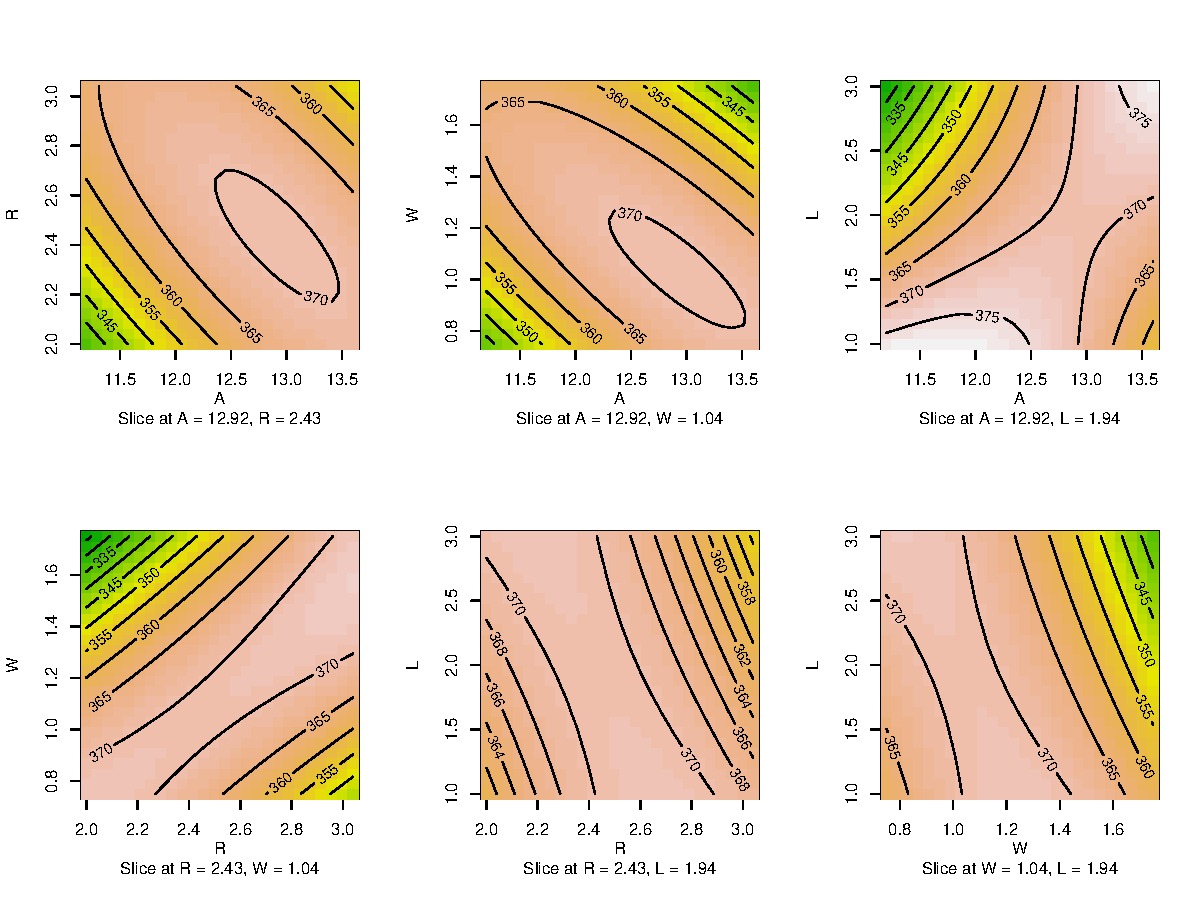
\includegraphics[width=.8\textwidth]{rsm-fig6.pdf}
\caption{\label{heliplots} Fitted response-surface contour plots near the stationary point for the helicopter experiment.}
\end{figure}
%
\section{Displaying a response surface}\label{contour}
While the canonical analysis gives us a handle on the behavior of a second-order response surface, an effective graph is a lot easier to present and explain.  To that end, "rsm" includes a function for making contour plots of a fitted response surface.  This function is not restricted to "rsm" results, however; it can be used for plotting any regression surface produced by "lm".  For more detailed information, see the associated vignette \href{rsm-plots.pdf}{``Surface Plots in the \rsm{} Package.''}
We provide the "lm" or "rsm" object, a formula for which predictors to use, and various optional parameters.  Consider the paper-helicopter example in the preceding section; there are four response-surface predictors, making six pairs of predictors.  If we want to visualize the behavior of the fitted surface around the stationary point, we can provide that location as the "at" argument:
\begin{Schunk}
\begin{Sinput}
R> par(mfrow = c(2, 3))
R> contour(heli.rsm, ~ x1 + x2 + x3 + x4, image = TRUE,
+   at = summary(heli.rsm)$canonical$xs)
\end{Sinput}
\end{Schunk}
The plots are shown in Figure~\ref{heliplots}.  The "image" argument causes each plot to display a color image overlaid by the
contour lines.  When multiple plots like this are produced, the color levels are held consistent across all
plots.  Note that the "at" condition does not set the center of the coordinate systems (the default variable
ranges are derived from the data); it sets the values at which to hold variables other than those on one of
the coordinate axes, as shown in the subtitles.


\section{Direction for further experimentation}\label{steepest}
In many first-order cases, as well as second-order cases where we find a saddle point or the stationary point is distant, the most useful further action is to decide in which direction to explore further.  In the case of first-order models, one can follow the direction of steepest ascent.  As already seen in \Sect{fitting}, the "summary" method for "rsm" objects provides some information about this path.  More detailed information is available via the "steepest" function; for example,
\begin{Schunk}
\begin{Sinput}
R> steepest(CR1.rsm, dist = c(0, 0.5, 1))
\end{Sinput}
\begin{Soutput}
Path of steepest ascent from ridge analysis:
  dist    x1    x2 |   Time    Temp |   yhat
1  0.0 0.000 0.000 | 85.000 175.000 | 82.814
2  0.5 0.407 0.291 | 87.035 176.455 | 83.352
3  1.0 0.814 0.581 | 89.070 177.905 | 83.890
\end{Soutput}
\end{Schunk}
In general, we can specify any set of distances along the path.  The  decoded coordinate values are displayed if the model was fitted to a "coded.data" dataset.  

At this point it is worth emphasizing that, although the fitted values are also displayed, one must be careful to understand that these are only predictions and that, as the distance increases, they are very poor predictions and should be taken with a grain of salt.  What one should do is to conduct actual experimental runs at points along this path, and use the observed response values, not these predictions, for guidance on where to locate the next factorial experiment.

In the second-order case, the "steepest" function still works, but it uses the ridge analysis method \cite[]{Hoe59,Dra63}, which is the analog of steepest ascent in the sense that for a specified distance $d$, it finds the point at which the predicted response is a maximum among all predictor combinations at radius $d$.  This method makes sense when the stationary point is some distance away; but when this point is nearby, it makes more sense to start at the saddle point (rather than the origin) and follow the most steeply rising ridge in \emph{both} directions.  This path is obtained using the "canonical.path" function.  In this function, distance is a signed quantity, according to the direction along the ridge.

In the "heli" example, we do have a nearby stationary point.  Here are some points within a radius of $5$ along the canonical path:
\begin{Schunk}
\begin{Sinput}
R> canonical.path(heli.rsm, dist = seq(-5, 5, by = 0.5))
\end{Sinput}
\begin{Soutput}
   dist     x1     x2     x3     x4 |       A       R       W      L |    yhat
1  -5.0 -1.728  1.921  1.419 -2.967 | 11.3632 3.01946 1.60475 0.5165 | 453.627
2  -4.5 -1.469  1.696  1.193 -2.682 | 11.5186 2.96096 1.54825 0.6590 | 438.150
3  -4.0 -1.210  1.471  0.967 -2.397 | 11.6740 2.90246 1.49175 0.8015 | 424.302
4  -3.5 -0.951  1.246  0.742 -2.112 | 11.8294 2.84396 1.43550 0.9440 | 412.094
5  -3.0 -0.692  1.021  0.516 -1.827 | 11.9848 2.78546 1.37900 1.0865 | 401.504
6  -2.5 -0.434  0.795  0.290 -1.541 | 12.1396 2.72670 1.32250 1.2295 | 392.534
7  -2.0 -0.175  0.570  0.064 -1.256 | 12.2950 2.66820 1.26600 1.3720 | 385.203
8  -1.5  0.084  0.345 -0.162 -0.971 | 12.4504 2.60970 1.20950 1.5145 | 379.502
9  -1.0  0.343  0.120 -0.388 -0.686 | 12.6058 2.55120 1.15300 1.6570 | 375.429
10 -0.5  0.602 -0.105 -0.614 -0.401 | 12.7612 2.49270 1.09650 1.7995 | 372.986
11  0.0  0.861 -0.331 -0.839 -0.116 | 12.9166 2.43394 1.04025 1.9420 | 372.172
12  0.5  1.120 -0.556 -1.065  0.169 | 13.0720 2.37544 0.98375 2.0845 | 372.987
13  1.0  1.378 -0.781 -1.291  0.454 | 13.2268 2.31694 0.92725 2.2270 | 375.428
14  1.5  1.637 -1.006 -1.517  0.739 | 13.3822 2.25844 0.87075 2.3695 | 379.499
15  2.0  1.896 -1.232 -1.743  1.024 | 13.5376 2.19968 0.81425 2.5120 | 385.206
16  2.5  2.155 -1.457 -1.969  1.309 | 13.6930 2.14118 0.75775 2.6545 | 392.538
17  3.0  2.414 -1.682 -2.195  1.594 | 13.8484 2.08268 0.70125 2.7970 | 401.498
18  3.5  2.673 -1.907 -2.421  1.879 | 14.0038 2.02418 0.64475 2.9395 | 412.088
19  4.0  2.932 -2.132 -2.646  2.164 | 14.1592 1.96568 0.58850 3.0820 | 424.295
20  4.5  3.190 -2.358 -2.872  2.449 | 14.3140 1.90692 0.53200 3.2245 | 438.140
21  5.0  3.449 -2.583 -3.098  2.734 | 14.4694 1.84842 0.47550 3.3670 | 453.615
\end{Soutput}
\end{Schunk}
\citet[Table~12.7 and~Figure~12.6]{Box05} reports some results of experimentation along this path.  They found the most promising location for the next experiment was at a distance of about $3.5$ ($-3.5$ on their scale as their signs are reversed from ours).

\section{Stationary and rising-ridge situations}
Canonical analysis becomes unstable in cases where the matrix $\bB$ of second-order coefficients is singular or nearly so. As an example, consider the dataset "codata" provided with \rsm{} and used as an example in \cite{Box05}. It comes in coded form, but to relate things to the actual variables, let's add the codings:
\begin{Schunk}
\begin{Sinput}
R> CO = as.coded.data(codata,  x1 ~ (Ethanol - 0.2)/0.1,  x2 ~ A.F.ratio - 15)
R> names(CO)[3] = "CO.conc"
R> head(CO)
\end{Sinput}
\begin{Soutput}
  Ethanol A.F.ratio CO.conc
1     0.1        14    61.9
2     0.1        14    65.6
3     0.2        14    80.9
4     0.2        14    78.0
5     0.3        14    89.7
6     0.3        14    93.8

Data are stored in coded form using these coding formulas ...
x1 ~ (Ethanol - 0.2)/0.1
x2 ~ A.F.ratio - 15
\end{Soutput}
\end{Schunk}
This is a $3^2$ design in one block. We fit a second-order model and obtain the canonical analysis:
\begin{Schunk}
\begin{Sinput}
R> CO.rsm = rsm(CO.conc ~ SO(x1,x2), data = CO)
R> canonical(CO.rsm)
\end{Sinput}
\begin{Soutput}
$xs
       x1        x2 
-14.81387  15.44149 

$eigen
$eigen$values
[1]  0.1868328 -8.8868328

$eigen$vectors
         [,1]       [,2]
x1  0.6893497 -0.7244288
x2 -0.7244288 -0.6893497
\end{Soutput}
\end{Schunk}
%
%--------------------- ILLUS FIGURE BEG --------------
\begin{figure}
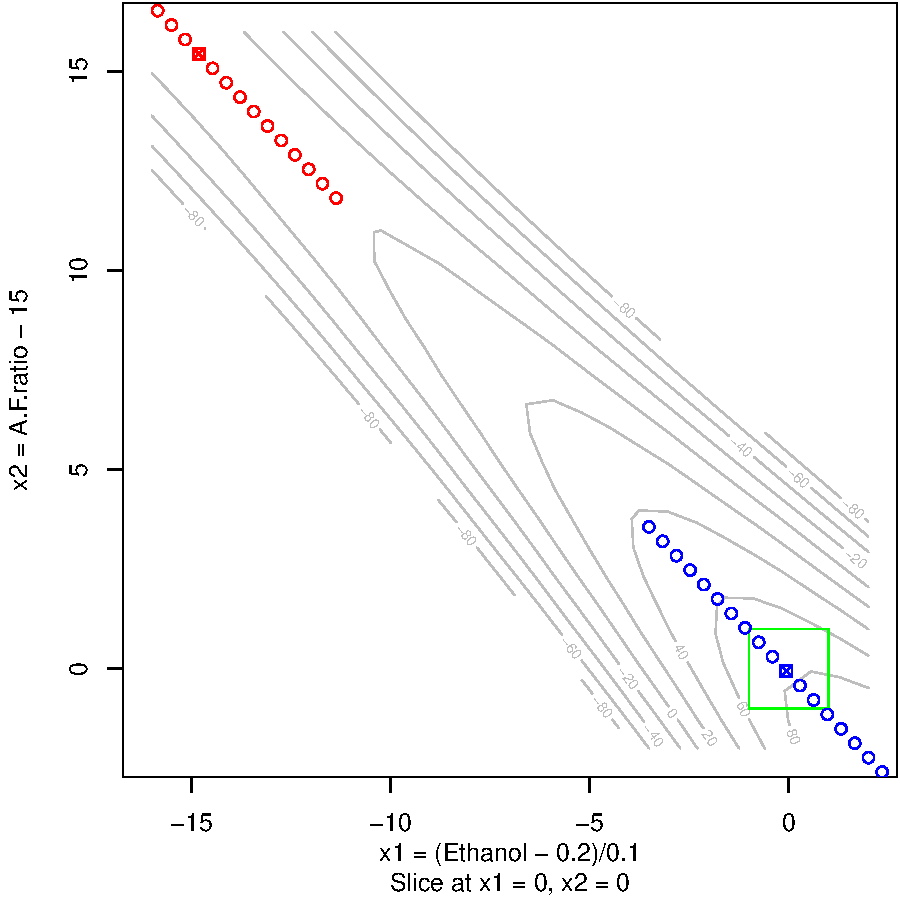
\includegraphics[width=.6\textwidth]{rsm-rising-ridge.pdf}

\caption{Fitted response surface for \code{CO.rsm}, and the canonical paths with (blue) and without(red) a threshold. The design region is shown as a green box.}\label{rising-ridge}
\end{figure}
%--------------------- ILLUS FIGURE END --------------
%
Note that the stationary point is at about $(-15,15)$ in coded units---very distant from the design center. Also, one eigenvalue is very small relative to the other. \rsm{} now provides a "threshold" option whereby eigenvalues smaller than the threshold are not used. Note the results when we discard the smaller eigenvalue:
\begin{Schunk}
\begin{Sinput}
R> canonical(CO.rsm, threshold = .2)
\end{Sinput}
\begin{Soutput}
$xs
         x1          x2 
-0.06302658 -0.05997463 

$eigen
$eigen$values
[1]  0.000000 -8.886833

$eigen$vectors
         [,1]       [,2]
x1  0.6893497 -0.7244288
x2 -0.7244288 -0.6893497
\end{Soutput}
\end{Schunk}
This sets the smaller eigenvalue to zero. By ignoring it, the stationary point is $(-.06,-.06)$---much, much closer to the design center. 

The following statements produce an illustrative plot, shown in Figure~\ref{rising-ridge}.
\begin{Schunk}
\begin{Sinput}
R> contour(CO.rsm, x2 ~ x1, bounds = list(x1=c(-16,2), x2=c(-2,16)), 
+         zlim=c(-100,100), col="gray", decode = FALSE)
R> lines(c(-1,1,1,-1,-1), c(-1,-1,1,1,-1), col="green") # design region
R> points(x2 ~ x1, data=canonical.path(CO.rsm), col="red", pch=1+6*(dist==0))
R> points(x2 ~ x1, data=canonical.path(CO.rsm, threshold=.2), 
+         col="blue", pch=1+6*(dist==0))
\end{Sinput}
\end{Schunk}
It displays the fitted response surface, as well as the results from "canonical.path" with and without the threshold (blue and red points, respectively). The region of the design is shown as a green box. The stationary point (different symbol) is seen to be a saddle point near the upper-left corner when not thresholded, and near the design center whern thresholded. Otherwise, the canonical paths are much the same but with different origins. Both form a path along the rising ridge that occurs in the vicinity of the design. 

It is important to note that the stationary point obtained by thresholding is not really a stationary point, but rather a nearby point that represents a center for the most important canonical directions. In this example, the true stationary point is very distant, and the thresholded stationary point is the nearest place on a rising ridge that emanates from the true stationary point. The thresholded "canonical.path" results give us a much more usable set of factor settings to explore than the ones without a threshold.

The rest of this section provides some technical backing, in case you're interested. Let $\bb$ and $\bB$ denote the first and second-order coefficients of the fitted second-order surface, so that the fitted value at a coded point $\bx$ is $\yhat(\bx) = b_0 + \bb'\bx + \bx'\bB\bx$. The stationary point $\bx_s$ solves the equation $2\bB\bx_s + \bb = \bzero$, i.e., $\bx_s = -\frac12\bB^{-1}\bb$. The canonical analysis yields the decomposition 
\[ \bB = \bU\bLambda\bU' = \lambda_1\bu_1\bu_1' + \lambda_2\bu_2\bu_2' + \cdots + \lambda_k\bu_k\bu_k' \]
where there are $k$ predictors, the $\bu_j$ form orthonormal columns of $\bU$, and the $\lambda_j$ are the eigenvalues, and $\bLambda = \mathrm{diag}(\lambda_1,\lambda_2,\ldots,\lambda_k)$. It also happens to be true that 
\[ \bB^{-1} = \bU\bLambda^{-1}\bU'
= \textstyle\frac1{\lambda_1}\bu_1\bu_1' + \frac1{\lambda_2}\bu_2\bu_2' + \cdots + \frac1{\lambda_k}\bu_k\bu_k'  \]
Thus, a really small value of $\lambda_j$ hardly affects $\bB$, but has a huge influence on $\bB^{-1}$.

Now, for some $m<k$, let $\bLambda_*$ be the $m\times m$ diagonal matrix with only some subset of $m$ eigenvalues; and let  $\bU_*$ be the $k \times m$ matrix with the corresponding $\bu_j$. If we excluded the smallest absolute eigenvalues, then $\bB_* = \bU_*\bLambda_*\bU'_* \approx \bB$. Moreover, by orthogonality, $\bU'\bB = \bLambda\bU'$ and $\bU_*'\bB = \bLambda_*\bU_*'$.
The stationary point satisfies $2\bB\bx + \bb = \bzero$ so that $2\bU_*'\bB\bx + \bU_*'\bb = \bzero$. Accordingly, we propose to define a pseudo-stationary point $\bx_*$ such that $2\bU_*'\bB\bx_* + \bU_*'\bb = \bzero$; i.e., $2\bLambda_*\bU_*'\bx_* + \bU_*'\bb = \bzero$. 

This comprises $m$ equations in $k>m$ unknowns. 
% To make it solvable, we can specify $\bgamme = \bU_0'\bx$ where $\bU_0$ consists of the $k-m$ columns of %$\bU$ not included in $\bU_*$. We now have the system of equations
% \[ 
% \bmat{ 2\bLambda_*\bU_*' \\ \bU_0' } \bx = \bmat{ -\bU_*'\bb \\ \bgamma}
% \]
% The question is which $\bgamma$ to choose. 
% We opt to choose the solution that is closest to the origin. 
To make it unique, we opt to choose the solution that is closest to the origin;
that is, minimize $\bx'\bx$ subject to the constraint that $2\bLambda_*\bU_*'\bx + \bU_*'\bb = \bzero$.
Using variational methods (Lagrange multipliers), we find that the resulting solution is $\bx_*= -\frac12\bU_*\bLambda_*^{-1}\bU_*'\bb$. In other words, we simply exclude some terms corresponding to small $\lambda_i$ in the above expression for $\bB^{-1}$.
This is the stationary point returned in \rsm's "canonical" and related functions when a threshold is used to exclude some small eigenvalues.


\section{Discussion}
The current version of \rsm{} provides only the most standard tools for first- and second-order response-surface design and analysis.  The package can be quite useful for those standard situations, and it implements many of the analyses presented in textbooks.  However, clearly a great deal of work has been done in response-surface methods that is not represented here.
Even a quick glance at a review article such as \cite{Mye04}---or even an older one such as \cite{Hil89}---reveals that there is a great deal that could be added to future editions of \rsm{}.  There are many other useful designs besides central composites and Box-Behnken designs.  We can consider higher-order models or the use of predictor transformations.  Mixture designs are not yet provided for.  There are important relationships between these methods and robust parameter design, and with computer experiments.  The list goes on.  However, we now at least have a good collection of basic tools for the \R{} platform, and that is a starting point.




\bibliography{rsm}

\end{document}
